	%-=-=-=-=-=-=-=-=-=-=-=-=-=-=-=-=-=-=-=-=-=-=-=-=
%
%        LOADING DOCUMENT
%
%-=-=-=-=-=-=-=-=-=-=-=-=-=-=-=-=-=-=-=-=-=-=-=-=

\documentclass[newPxFont,pagenumber]{beamer}
\usetheme{sthlm}
%\usecolortheme{sthlmv42}

%-=-=-=-=-=-=-=-=-=-=-=-=-=-=-=-=-=-=-=-=-=-=-=-=
%        LOADING PACKAGES
%-=-=-=-=-=-=-=-=-=-=-=-=-=-=-=-=-=-=-=-=-=-=-=-=
\usepackage[utf8]{inputenc}
\usepackage[frenchb]{babel}
\usepackage[normalem]{ulem}
\usepackage{caption}
\captionsetup{font=scriptsize}
%\usepackage[font=footnotesize]{subcaption}
% in preamble
\usepackage{chronology}
\usepackage{pgf}
\usepackage{tikz}
\usetikzlibrary{arrows,automata}
\usepackage{array,multirow}
\usepackage{nameref}
\makeatletter
\newcommand*{\currentname}{\@currentlabelname}
\makeatother

\graphicspath{ {fig/} }

\usepackage[linesnumbered,ruled,vlined]{algorithm2e}
% add page number
%\usepackage[defaultsans]{cantarell}

\newcommand{\p}{\mathbb{P}}

\setbeamerfont{title}{series=\upshape}
\setbeamertemplate{footline}{\hfill\footnotesize\insertframenumber\hskip3pt\null\vskip3pt}

\newcommand{\argmax}{\mathop{\mathrm{argmax}}\limits}
\renewcommand{\max}{\mathop{\mathrm{max}}\limits}

\renewcommand{\event}[3][e]{%
  \pgfmathsetlength\xstop{(#2-\theyearstart)*\unit}%
  \ifx #1e%
    \draw[fill=black,draw=none,opacity=0.5]%
      (\xstop, 0) circle (.2\unit)%
      node[opacity=1,rotate=45,right=.2\unit] {#3};%
  \else%
    \pgfmathsetlength\xstart{(#1-\theyearstart)*\unit}%
    \draw[fill=black,draw=none,opacity=0.5,rounded corners=.1\unit]%
      (\xstart,-.1\unit) rectangle%
      node[opacity=1,rotate=45,right=.2\unit] {#3} (\xstop,.1\unit);%
  \fi}%

\addto\captionsfrench{%
\renewcommand{\figurename}{\scriptsize {\scshape Figure}}
\renewcommand{\tablename}{\scriptsize {\scshape Table}}
}

%-=-=-=-=-=-=-=-=-=-=-=-=-=-=-=-=-=-=-=-=-=-=-=-=
%        BEAMER OPTIONS
%-=-=-=-=-=-=-=-=-=-=-=-=-=-=-=-=-=-=-=-=-=-=-=-=

%\setbeameroption{show notes}
\setbeamersize{text margin left=5pt,text margin right=5pt}

%-=-=-=-=-=-=-=-=-=-=-=-=-=-=-=-=-=-=-=-=-=-=-=-=
%
%	PRESENTATION INFORMATION
%
%-=-=-=-=-=-=-=-=-=-=-=-=-=-=-=-=-=-=-=-=-=-=-=-=

\title{\vspace{0.4cm}\normalsize Extraction des demandes dans les décisions jurisprudentielles} 
\subtitle{
\scriptsize séminaire LGI2P, IMT Mines Alès -- \textit{15 mars 2018}
}
%\date{\small{\jobname}}
\date{\scriptsize Début de thèse: 15 Décembre 2015}
\author{
%\normalsize Gildas Tagny Ngompé
}
\institute{\scriptsize 
\textbf{Doctorant:} Gildas Tagny Ngompé

\textbf{Direction de thèse:} \begin{itemize}
\item Jacky Montmain (École des mines d'Alès, LGI2P)
\item Stéphane Mussard (Université de Nîmes, CHROME)
\end{itemize}
\textbf{Encadrement de proximité:} \begin{itemize}
\item Sébastien Harispe (Ecole des Mines d'Alès, LGI2P)
\item Guillaume Zambrano (Université de Nîmes, CHROME)
\end{itemize}}

\hypersetup{
pdfauthor = {\author{}: tagnyngompe@gmail.com},
pdfsubject = {},
pdfkeywords = {},
pdfmoddate= {D:\pdfdate},
pdfcreator = {}
}

\begin{document}
\nocite{}
%-=-=-=-=-=-=-=-=-=-=-=-=-=-=-=-=-=-=-=-=-=-=-=-=
%
%	TITLE PAGE
%
%-=-=-=-=-=-=-=-=-=-=-=-=-=-=-=-=-=-=-=-=-=-=-=-=
\begin{frame}[plain]
	\titlepage
\end{frame}
%}
%-=-=-=-=-=-=-=-=-=-=-=-=-=-=-=-=-=-=-=-=-=-=-=-=
%
%	TABLE OF CONTENTS: Plan
%
%-=-=-=-=-=-=-=-=-=-=-=-=-=-=-=-=-=-=-=-=-=-=-=-=
\section*{Plan}
\begin{frame}[c]{\currentname}
\tableofcontents[hideallsubsections]
\end{frame}

\section{Motivations et objectifs}

\begin{frame}[c]{Les juristes analysent les décisions}
\begin{center}
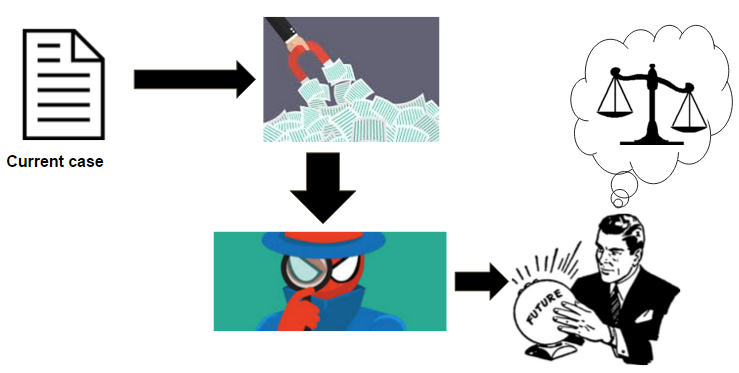
\includegraphics[width=0.7\textwidth]{lawyerwork.png}
\end{center}

\begin{block}{Pourquoi?}
\begin{itemize}
\item comprendre et comparer l'application loi (contentieux, ville, ...)
\item estimer le risque judiciaire
\item ... %anticiper les affaires futures
\end{itemize}
\end{block}
\end{frame}

\begin{frame}{Motivation: documents non-structurés, langage complexe}
\scriptsize
\begin{columns}
\begin{column}{.50\linewidth}
ARRÊT N°

R.G: 11/03924

...

{COUR D'APPEL} DE {NÎMES}

{CHAMBRE CIVILE}

{1ère Chambre A}

ARRÊT DU {20 MARS 2012}

APPELANTE:

{Madame Michéle A.} ...

assistée de la {SELARL VAJOU}, ...

INTIMES:

{Monsieur Martial B} ...

assisté de la {SCP MARION GUIZARD PATRICIA SERVAIS}, ...

COMPOSITION DE LA COUR LORS DU DÉLIBÉRÉ:

{M. Dominique BRUZY, Président}

{M. Serge BERTHET, Conseiller}

...
\end{column}
\begin{column}{.50\linewidth}
FAITS, PROCEDURE, ...

Madame Michèle A. demande:

...

- de condamner Madame JONES-B. à lui payer la somme de {2.500 euros} au titre de l'{article 700 du Code de Procédure Civile}, 

\vspace{0.4cm}

PAR CES MOTIFS, LA COUR:

...

Vu l'{article 809 du Code de Procédure Civile},

...

{Déboute Madame A. de sa demande de provision sur dommages-intérêts.}

...

Vu l'{article 700 du Code de Procédure Civile},

Condamne Madame JONES-B. à verser à Madame A. la somme de {2.500 euros}.
\end{column}
\end{columns}
\end{frame}

\begin{frame}[c]{Motivation: grand volume de décisions}
\textbf{Plus de 4 millions de décisions prononcées / an}
\begin{table}[!htb]
{
\footnotesize
\begin{center}
\begin{tabular}{|p{2cm}|c|c|c|c|c|}
\hline
 & \textbf{2010} & \textbf{2011} & \textbf{2012} & \textbf{2013} & \textbf{2014} \\
 \hline
 \textbf{Justice civile} & 2 673 131  & 2 654 179 & 2 647 813 & 2 761 554  & 2 618 374 \\
 \hline
Justice pénale & 1 173 242 & 1 180 586 & 1 251 979 & 1 303 469 & 1 203 339 \\
 \hline
 Justice administrative & 224 787 & 225 608 & 228 680 & 221 882 & 230 477 \\
 \hline
\end{tabular}

\textit{\tiny{Source: \url{http://www.justice.gouv.fr/budget-et-statistiques-10054/chiffres-cles-de-la-justice-10303/}}}  
\end{center}
}
\caption{Nombre de décisions prononcées en France par an}\label{decisionstats}
\end{table}
\end{frame}

\begin{frame}[t]{Motivation: recherches et analyses sémantiques difficiles}

Moteurs de recherche juridique à mots-clés 

Pas d'analyse synthétique des décisions 

%\begin{figure}
\fbox{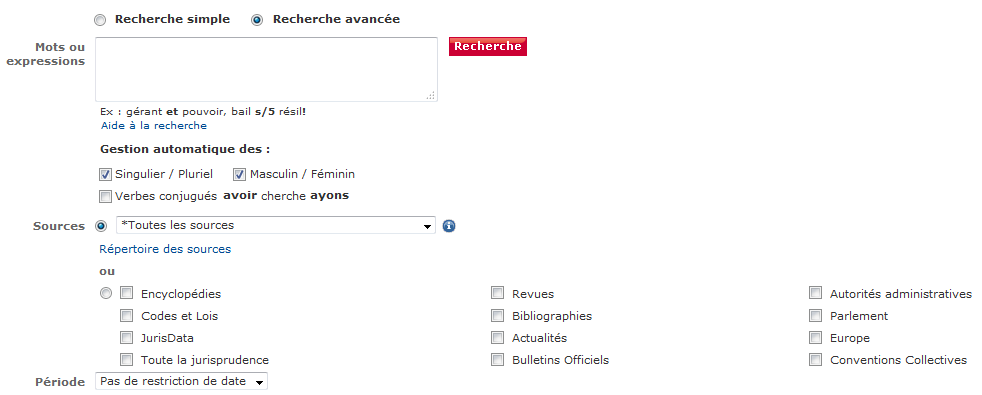
\includegraphics[width=0.9\paperwidth]{jurica.png}}

\textit{\tiny{Source: \url{LexisNexis.com}}} 
%\caption{Formulaire de recherche}
%\end{figure}
\end{frame}

\begin{frame}{Proposition: Moteur d'analyse sémantique de corpus}
Stage été 2017 [ PRYSIAZHNIUK Anastasiia ]
\begin{center}
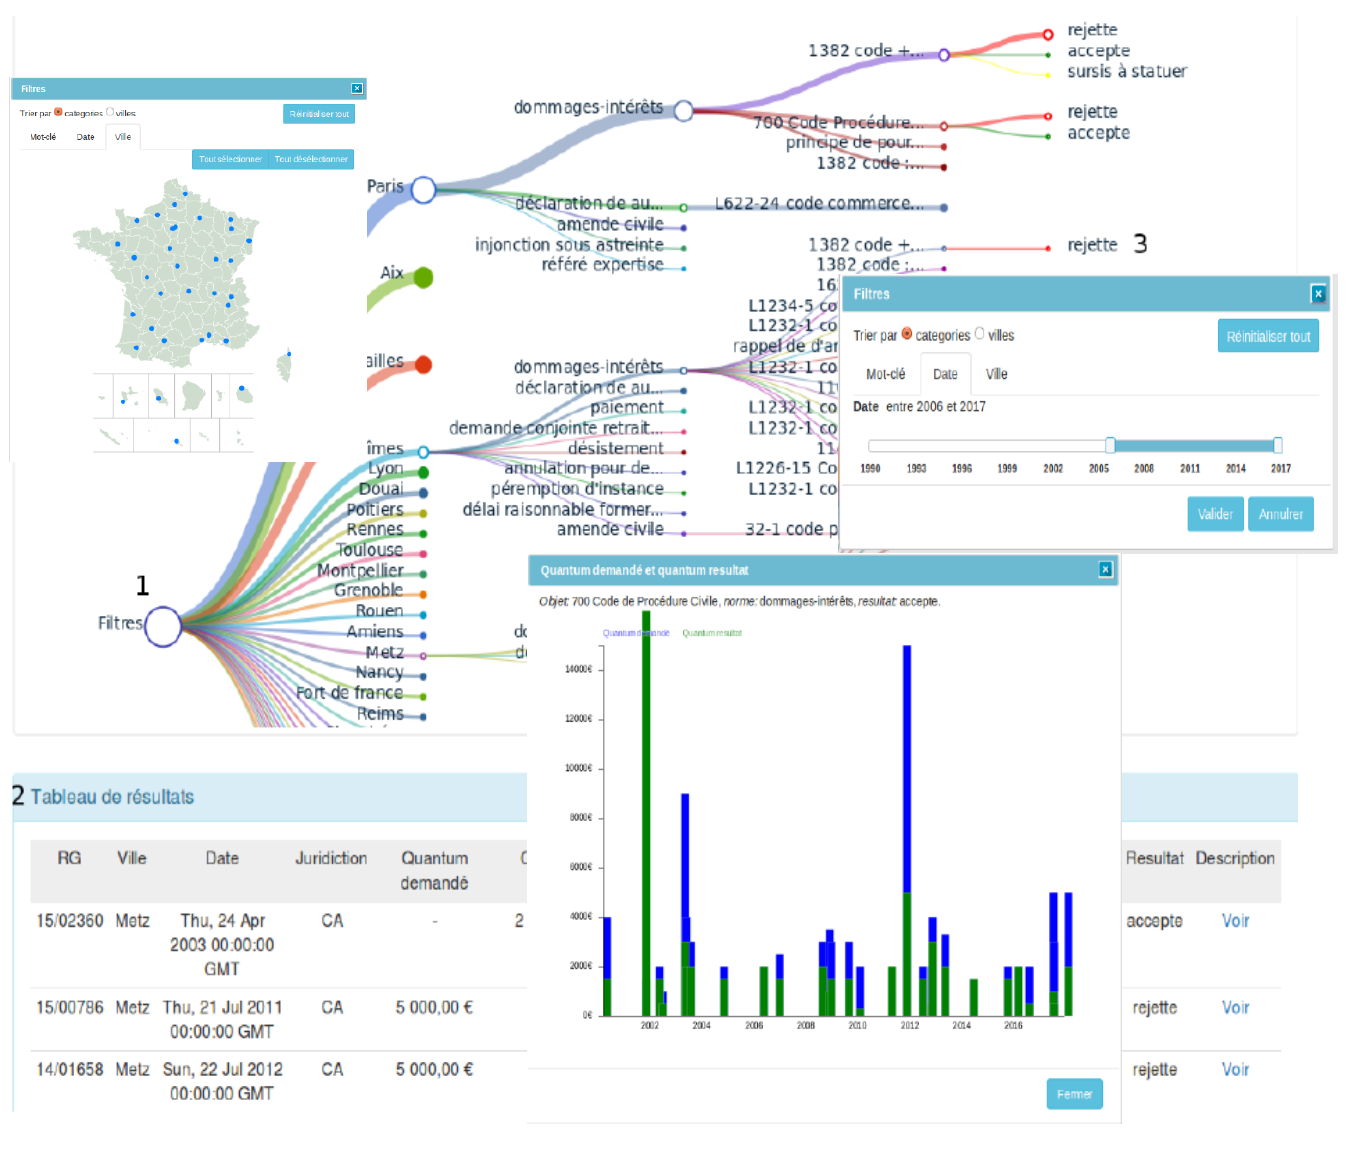
\includegraphics[width=0.75\textwidth]{interface.png}
\end{center}
\end{frame}

\begin{frame}{Pipeline d'analyse sémantique}
\centering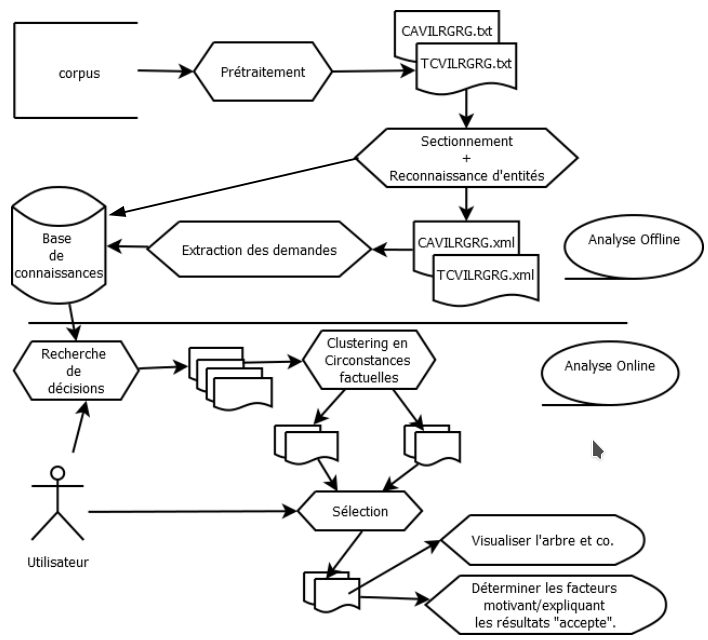
\includegraphics[width=0.75\textwidth]{pipelineComplet.png}
\end{frame}

\begin{frame}{Phase actuelle: extraction d'information}
\centering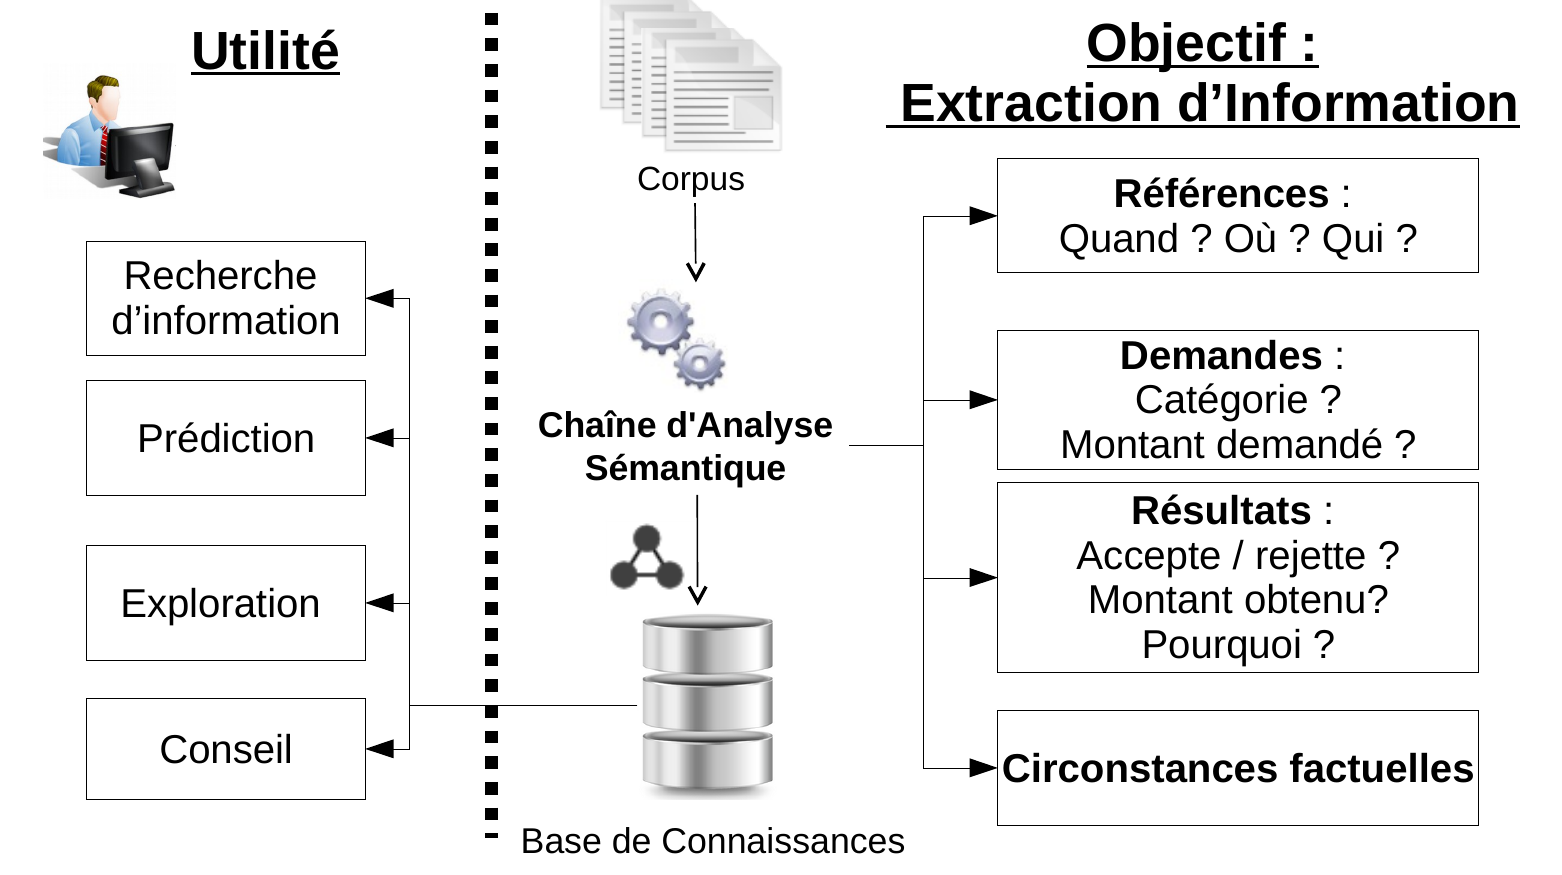
\includegraphics[width=\textwidth]{summary-prj.png}
\end{frame}

\section{Extraction d'information sur les demandes et  résultats}

\begin{frame}{T\^ache: extraire les quanta et le sens du résultat}
\begin{table}
\centering 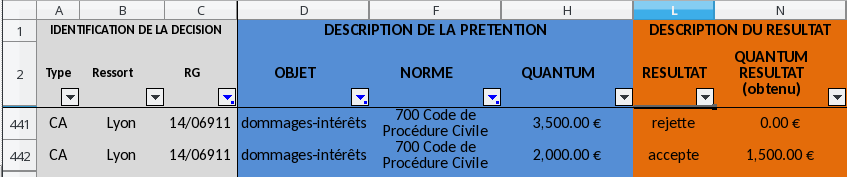
\includegraphics[width=\textwidth]{tab-annotations.png}
\caption{\scriptsize Tableau des informations sur les demandes}
\end{table}

\begin{exampleblock}{Exemple: Informations pertinentes à extraire}%CAANG1500238.xml
\begin{itemize}\scriptsize
%\item \textbf{Position de la partie}: Intimé
\item \textbf{Catégorie prédéfinie}: Dommages-intérêts pour procédure abusive
\begin{itemize}\scriptsize
\item \textbf{Objet}: Dommages-intérêts
\item \textbf{Fondement}: Articles 1382 code civil et 32-1 code de procédure civile
\end{itemize}
\item \textbf{Quantum demandé}: 20 000 euros
\item \textbf{Sens du résultat} : "\textit{rejette}"
\item \textbf{Quantum accordé} : 0 euros
\end{itemize}
\end{exampleblock}
\end{frame}

\begin{frame}{Difficultés (1)}
%\small
Expressions non structurées, par  \textcolor{orange}{référence}, par \textcolor{blue}{agrégation}

\begin{exampleblock}{Exemple (suite): Expression de demande} % CAANG1500238.xml
La société A. conclut à la confirmation du jugement entrepris sauf à
former appel incident sur la disposition du jugement l'ayant déboutée de sa
demande de \textbf{dommages-intérêts pour abus de procédure} et elle demande à la cour de
condamner l'appelante à lui payer la somme de \textbf{20 000 euros} à titre de dommages
intérêts ...

\end{exampleblock}

\begin{exampleblock}{Exemple (suite): Expression de resultat}
La cour, ... 

Confirme \textcolor{orange}{la décision entreprise} en \textcolor{blue}{toutes ses dispositions},
\end{exampleblock}
\end{frame}

\begin{frame}{Difficultés (2)}
\begin{alertblock}{}
\begin{itemize}
\item Présence de plusieurs demandes de catégories similaires et/ou différentes dans une m\^eme décision
\item Toutes les catégories ne sont pas connues d'avance (+500 catégories)
\item Difficile d'annoter une base d'évaluation pour toutes les couvrir
\end{itemize}
\end{alertblock}

\begin{block}{Il faut une approche :}
\begin{itemize}
\item qui s'adapte à la catégorie à extraire 
\item qui permette de rajouter de nouvelles catégories 
\end{itemize}
\end{block}
\end{frame}
\section{Une approche basée sur la pondération de termes et le zonage}
\begin{frame}{Architecture du pipeline d'extraction}
\begin{figure}
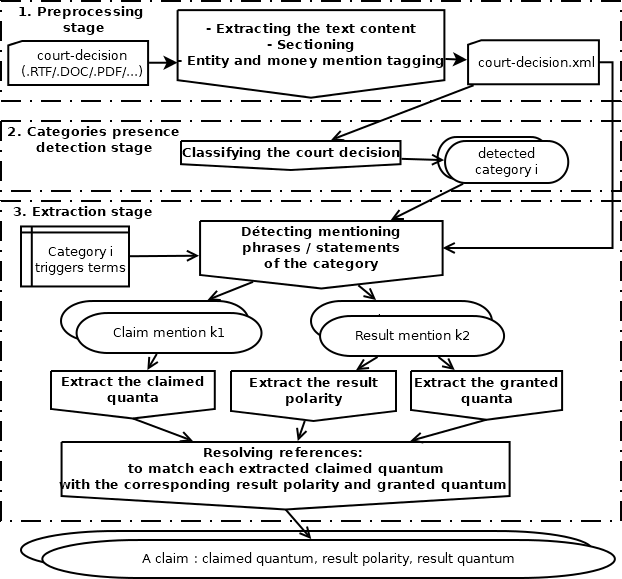
\includegraphics[width=0.7\textwidth]{pipeline-dmd.png}
\caption{Pipeline d'extraction d'analyse.}
\end{figure}
\end{frame}

\begin{frame}{Identification des passages et des informations}
Demande dans la section \textit{Litige} (Faits, procédures, et moyens des parties)

Résultat dans la section \textit{Dispositif}
\scriptsize
\begin{table}
 \begin{tabular}{|p{0.28\textwidth}|p{0.3\textwidth}|p{0.12\textwidth}|p{0.11\textwidth}|}
 \hline
 \textbf{Demande} & \multicolumn{3}{c|}{\textbf{Résultat} (organisé par polarité)} \\ \hline
  & \textbf{accepte}  &\textbf{sursis à statuer} & \textbf{rejette}  \\ \hline
 \textit{accorder, admettre, admission, allouer, condamnation, condamner, fixer, laisser, prononcer, ramener, surseoir} & \textit{accorde, accordons, admet, admettons, alloue, allouons, condamne, condamnons, déclare, déclarons, fixe, fixons, laisse, laissons, prononce, prononçons} & \textit{réserve, réservons, surseoit, sursoyons} & \textit{déboute, déboutons, rejette, rejettons} \\ \hline
 \end{tabular}
  \caption{Mots introduisant les énoncés de demandes et de résultats}\label{introducing-words}
 \end{table}
 
 
 \begin{figure}
 \begin{flushleft}
%" ... débouter M. S. de l' ensemble de ses demandes

- le \textbf{<demande categorie="acpa">}\underline{condamner} à payer une <trigger categorie="acpa">\textbf{amende civile}</trigger> de <argent> \textbf{1.500 euros} </argent> pour procédure abusive ...

- le\textbf{</demande>} \underline{condamner} à payer la somme ..."
\end{flushleft}
\caption{Exploiter la proximité entre triggers et sommes d'argent}\label{example-zone}
\end{figure} 
\end{frame}

\begin{frame}{Identification des passages et des informations(2)}
\begin{itemize}
\item Identification des passages: 
\begin{enumerate}
\item Soit par la seule \textbf{présence d'un trigger} : on zone autour des triggers 
\item Soit par \textbf{pondération des zones à argent}  : 
\begin{enumerate}
\item on zone autour des sommes d'argent
\item on pondère les zones (par ex. somme des poids des triggers)
\item on sélectionne une zone si elle a un poids $\geq$ \texttt{POIDS SEUIL}
\end{enumerate}
\end{enumerate}
\item Identification des informations:
\begin{enumerate}
\item quantum: somme d'argent près d'un trigger
\item sens du résultat : 
\begin{itemize}
\item soit en fonction du verbe introductif de l'énoncé du résultat
\item soit "\textit{rejette}" si pas d'énoncé du résultat
\end{itemize}
\end{enumerate}
\item Résolution des références:
\begin{itemize}
\item matching des énoncés (similarité textuelle)
\item matching des quanta (Hypothèse d'apparition dans le même ordre)
\end{itemize}
\end{itemize}
\end{frame}

\begin{frame}{Phase d'entrainement}
Catégorie  $c_i$, Corpus d'entrainement  $D = D_{c_i} \cup D_{\overline{c_i}} = \lbrace D_j\rbrace_{1\leq j\leq \vert D \vert}$
\begin{enumerate}
\item \textbf{Détecteur de catégorie: }
\begin{itemize}
\item vectoriser les décisions de la base d'entrainement: $w(t_k, D_j) = lw(t_k, D_j) \times gw(t_k) \times nf(D_j)$ \cite{salton1988term-weighting}
\item entrainer un algorithme de classification  (SVM, Naïf Bayésien, K plus proches voisins ...)
\end{itemize}
\item \textbf{Extracteur de triplets de quanta et sens du résultat:}
\begin{itemize}
\item Apprendre les triggers sur la base d'entrainement (passages à quanta vs. passages sans quanta)
\begin{enumerate}
\item pondération des termes $t_k$ avec une métrique de RI par ex. :

\text{Métrique non supervisée: } 

 $idf(t_k) = \log_2 (\frac{N}{N_{t_k}})$  \cite{sparck1972idf}

\text{Métriques supervisées : } 

 $gss(t_k,c_i) = (N_{t_k,c_i} N_{\overline{t_k},\overline{c_i}}) -  (N_{t_k,\overline{c_i}} N_{\overline{t_k},c_i})$ \cite{galavotti2000gss}

 $ngl(t_k,c_i) = \frac{\sqrt{N} ((N_{t_k,c_i} N_{\overline{t_k},\overline{c_i}}) - (N_{t_k,\overline{c_i}} N_{\overline{t_k},c_i}))}{\sqrt{N_{t_k} N_{\overline{t_k}} N_{c_i} N_{\overline{c_i}}}}$ \cite{ng1997ngl}
\item ranking puis sélection 
\end{enumerate}
\end{itemize}
\end{enumerate}
\end{frame}

\section{Expérimentations et résultats}
\subsection{Protocole d'évaluation}
\subsection{Données}
\begin{frame}{Données}
\begin{figure}
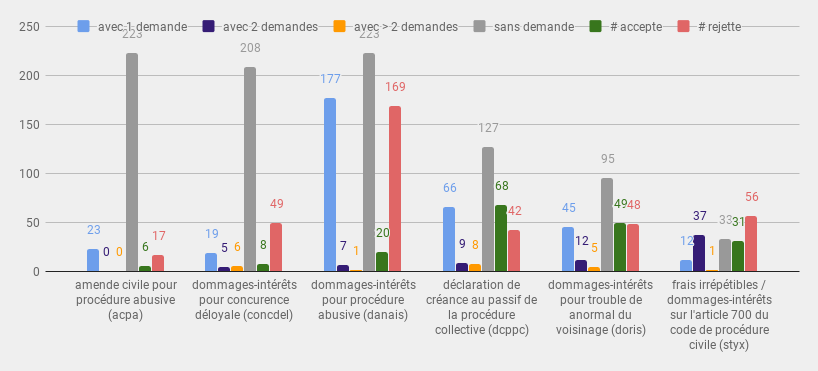
\includegraphics[width=\textwidth]{chartDataset.png}
\caption{Répartitions des demandes dans les documents annotées pour chaque catégorie.}
\end{figure}
\end{frame}

\begin{frame}{Métriques d'évaluation}
Catégorie  $c_i$, tuple d'information $I \subseteq \lbrace Q_{DMD}, S_{RST}, Q_{RST} \rbrace $

Corpus d'évaluation  $D = D_{c_i} \cup D_{\overline{c_i}} = \lbrace D_j\rbrace_{1\leq j\leq \vert D \vert}$, où $D_j$  est un document

\scriptsize
\[\text{Nombre de vrais positifs (bons): } TP_{c_i,I,D} = \sum\limits^{\vert D \vert}_{j=1} TP_{c_i,I,D_j}\] 
\[\text{Nombre de faux positifs (en trop): } FP_{c_i,I,D} = \sum\limits^{\vert D \vert}_{j=1} FP_{c_i,I,D_j}\] 
\[\text{Nombre de faux négatifs (manqués): } FN_{c_i,I,D_j} = \sum\limits^{\vert D \vert}_{j=1} FN_{c_i,I,D_j}\]
\[Precision_{c_i,I,D} = \frac{TP_{c_i,I,D}}{TP_{c_i,I,D} + FP_{c_i,I,D}}\]
\[Rappel_{c_i,I,D} = \frac{TP_{c_i,I,D}}{TP_{c_i,I,D} + FN_{c_i,I,D}}\]

\[F1_{c_i,I,D} =2 \times \frac{Precision_{c_i,I,D} \times Rappel_{c_i,I,D}}{Precision_{c_i,I,D} + Rappel_{c_i,I,D}}\]


\end{frame}

\begin{frame}{Evaluation de la détection des catégories}
\begin{table}
\tiny
\caption{Resultats d'une 5-fold cross-validation sur $D$ pour la detection categorie  à l'aide de Weka \cite{frank2016weka}  (P= Precision, R=Rappel, F1 = F1-mesure)}\label{best_classif_score}
\begin{tabular}{l|c@{\hskip 0.1in}lllc@{\hskip 0.1in}lllc@{\hskip 0.1in}lllc@{\hskip 0.1in}lll}
\hline\noalign{\smallskip}
       &   \multicolumn{3}{c}{Naïf Bayésien}    &    \multicolumn{3}{c}{Arbre de décision (J48)}   &  \multicolumn{3}{c}{KNN}  & \multicolumn{3}{c}{SVM}     \\       
\noalign{\smallskip}
\hline
\noalign{\smallskip}
  Category      & P     & R     & F1    & P     & R     & F1    & P     & R     & F1    & P     & R     & F1    \\        
\noalign{\smallskip}
\hline
\noalign{\smallskip}
acpa    & 1.0 & 1.0 & 1.0 & 0.996 & 0.955 & 0.972 & 1.0 & 1.0 & 1.0 & 0.996 & 0.955 & 0.972 \\
concdel & 1.0 & 1.0 & 1.0 & 1.0 & 1.0 & 1.0 & 1.0 & 1.0 & 1.0 & 0.995 & 0.967 & 0.979 \\
danais  & 0.988 & 0.989 & 0.988 & 0.996 & 0.995 & 0.995 & 0.995 & 0.995 & 0.995 & 0.993 & 0.993 & 0.993 \\
dcppc   & 1.0 & 1.0 & 1.0 & 1.0 & 1.0 & 1.0 & 1.0 & 1.0 & 1.0 & 1.0 & 1.0 & 1.0 \\
doris   & 1.0 & 1.0 & 1.0 & 1.0 & 1.0 & 1.0 & 1.0 & 1.0 & 1.0 & 1.0 & 1.0 & 1.0 \\
styx    & 1.0 & 1.0 & 1.0 & 0.984 & 0.983 & 0.983 & 1.0 & 1.0 & 1.0 & 1.0 & 1.0 & 1.0 \\
\hline
\end{tabular}
\end{table}
\end{frame}

\begin{frame}{Quelle pondération des triggers et quel  zonage?}
\begin{table}[]
\tiny
\begin{flushleft}
\caption{Comparaison des métriques de pondération et des stratégies de zonage sur le corpus $D$ (F1-mesure sur l'extraction du tuple $(Q_{DMD},S_{RST}, Q_{RST})$)}
\label{my-label}
\begin{tabular}{l|ll|ll|ll|ll|ll|ll}
Métrique & \multicolumn{2}{c|}{acpa} &  \multicolumn{2}{c|}{concdel}  &  \multicolumn{2}{c|}{danais} &  \multicolumn{2}{c|}{dcppc} &  \multicolumn{2}{c|}{doris}   &  \multicolumn{2}{c}{styx}    \\ \noalign{\smallskip}
\hline
         & tp    & zw    & tp      & zw    & tp     & zw    & tp    & zw    & tp    & zw    & tp    & zw    \\ \noalign{\smallskip}
\hline
CHI2     & 0.683 & 0.698 & 0.061   & 0.061 & 0.443  & 0.411 & 0.259 & 0.264 & 0.187 & 0.071 & 0.321 & 0.366 \\
DBIDF    & 0.683 & 0.698 & 0.076   & 0.033 & 0.461  & 0.416 & 0.254 & 0.264 & 0.084 & 0     & 0.331 & 0.358 \\
DELTADF  & 0.683 & 0.698 & 0.144   & 0.082 & 0.443  & 0.41  & 0.259 & 0.264 & 0.143 & 0.142 & 0.334 & 0.281 \\
DSIDF    & 0.678 & 0.698 & 0.076   & 0.052 & 0.399  & 0.152 & 0.014 & 0     & 0.019 & 0     & 0.343 & 0.33  \\
GSS      & 0.683 & 0.698 & 0.144   & 0.082 & 0.443  & 0.41  & 0.259 & 0.264 & 0.143 & 0.142 & 0.334 & 0.281 \\
IDF      & 0.067 & 0     & 0.033   & 0     & 0.04   & 0     & 0     & 0     & 0     & 0     & 0     & 0     \\
IG       & 0.011 & 0.049 & 0.05    & 0.034 & 0.304  & 0.073 & 0     & 0     & 0.019 & 0     & 0.058 & 0     \\
KLD      & 0.432 & 0.398 & 0.146   & 0.124 & 0.459  & 0.409 & 0.252 & 0.254 & 0.158 & 0.154 & 0.243 & 0.42  \\
MAR      & 0.683 & 0.698 & 0.144   & 0.091 & 0.443  & 0.42  & 0.259 & 0.264 & 0.156 & 0.146 & 0.334 & 0.281 \\
NGL      & 0.683 & 0.698 & 0.061   & 0.034 & 0.443  & 0.411 & 0.259 & 0.264 & 0.122 & 0.02  & 0.321 & 0.347 \\
RF       & 0.683 & 0.698 & 0.202   & 0.043 & 0.491  & 0.367 & 0.242 & 0.21  & 0.101 & 0.058 & 0.387 & 0.351 \\ \hline
 \noalign{\smallskip}
\hline
Max        & 0.683 & \textbf{0.698} & \textbf{0.202}   & 0.124  & \textbf{0.491}  & 0.42  & 0.259 & \textbf{0.264} & \textbf{0.187} & 0.154 & 0.387 & \textbf{0.42} 
\end{tabular}

tp = zonage par la seule présence d'un trigger

zw = zonage par pondération des passages à somme d'argent
\end{flushleft}

\end{table}

La métrique et la stratégie de zonage dépendent de la catégorie

\end{frame}

\begin{frame}{Exemple de termes sélectionnés}
\scriptsize
\begin{table}
\begin{tabular}{ll|lp{0.28\textwidth}}
 \multicolumn{2}{c|}{concdel} &  \multicolumn{2}{c}{danais} \\ \hline \noalign{\smallskip}
 NGL & DSIDF & NGL & DSIDF \\ \hline
déloyale & concurrence déloyale & procédure abusive       & procédure abusive et injustifiée                  \\ \hline
perte    & déloyale             & 32-1                    & fondement de l ' article 32-1                     \\ \hline
actes    &                      & abusive                 & dommages-intérêts pour procédure abusive          \\ \hline
50.000   & agissements          & intérêts pour procédure & titre de dommages-intérêts pour procédure abusive
\end{tabular}
\end{table}

$ngl(t_k,c_i) = \frac{\sqrt{N} ((N_{t_k,c_i} N_{\overline{t_k},\overline{c_i}}) - (N_{t_k,\overline{c_i}} N_{\overline{t_k},c_i}))}{\sqrt{N_{t_k} N_{\overline{t_k}} N_{c_i} N_{\overline{c_i}}}}$

$dsidf(t_k, c_i)=\log (\frac{(N_{\overline{c_i}}N_{t_k,c_i}) + 0.5}{(N_{c_i}N_{t_k,\overline{c_i}}) + 0.5} $
\end{frame}

\begin{frame}{Entrainement avec sélection de la meilleure métrique (1)}
\begin{table}[!htbp]
\tiny
\begin{tabular}{|c|c|c|c|c|c|c|}
\hline
$c_i$ & Tuple d'info ($I$) &  $P_{c_i,I,D_{c_i}}$ & $R_{c_i,I,D_{c_i}}$ & $F1_{c_i,I,D_{c_i}}$ & Docs. Parfaits & \#extraits/\#attendus/$\vert D_{c_i}  \vert$\\ \hline
\multirow{4}{*}{acpa} & $(Q_{DMD})$ & 0.709 & 0.73 & 0.705 & \textcolor{red}{0.47} & \multirow{5}{*}{5.2/4.6/4.6} \\ 
 & $(S_{RST})$ & 0.691 & 0.7 & 0.683 & \textcolor{red}{0.48} &  \\ 
 & $(Q_{RST})$ & 0.72 & 0.74 & 0.716 & \textcolor{red}{0.48} &  \\ 
 & $(Q_{DMD},S_{RST}, Q_{RST})$ & 0.651 & 0.65 & 0.638 & \textcolor{red}{0.43} &  \\  \hline
\multirow{4}{*}{concdel}  & $(Q_{DMD})$ & \textcolor{red}{0.461} & \textcolor{red}{0.393} & \textcolor{red}{0.376} & \textcolor{red}{0.233} & \multirow{5}{*}{11.6/11.6/6.0} \\ 
 & $(S_{RST})$ & 0.544 & \textcolor{red}{0.442} & \textcolor{red}{0.427} & \textcolor{red}{0.2} &  \\ 
 & $(Q_{RST})$ & 0.595 & \textcolor{red}{0.482} & \textcolor{red}{0.465} & \textcolor{red}{0.2} &  \\ 
 & $(Q_{DMD},S_{RST}, Q_{RST})$ & \textcolor{red}{0.337} & \textcolor{red}{0.299} & \textcolor{red}{0.28} & \textcolor{red}{0.167} &  \\  \hline
 \multirow{4}{*}{danais} & $(Q_{DMD})$ & 0.548 & 0.516 & 0.527 & \textcolor{red}{0.346} & \multirow{4}{*}{36.6/38.8/37.0} \\ 
 & $(S_{RST})$ & 0.69 & 0.646 & 0.661 & \textcolor{red}{0.454} &  \\ 
 & $(Q_{RST})$ & 0.714 & 0.666 & 0.682 & \textcolor{red}{0.465} &  \\ 
 & $(Q_{DMD},S_{RST}, Q_{RST})$ & \textcolor{red}{0.482} & \textcolor{red}{0.46} & \textcolor{red}{0.466} & \textcolor{red}{0.314} &  \\  \hline
\multirow{4}{*}{dcppc} & $(Q_{DMD})$ & \textcolor{red}{0.334} & \textcolor{red}{0.392} & \textcolor{red}{0.358} & \textcolor{red}{0.217} & \multirow{4}{*}{26.8/22.2/16.6} \\ 
 & $(S_{RST})$ & 0.665 & 0.798 & 0.721 & 0.544 &  \\ 
 & $(Q_{RST})$ & 0.62 & 0.744 & 0.672 & 0.509 &  \\ 
 & $(Q_{DMD},S_{RST}, Q_{RST})$ & \textcolor{red}{0.22} & \textcolor{red}{0.26} & \textcolor{red}{0.237} & \textcolor{red}{0.181} &  \\  \hline
 \multirow{4}{*}{doris} & $(Q_{DMD})$ & \textcolor{red}{0.279} & \textcolor{red}{0.373} & \textcolor{red}{0.314} & \textcolor{red}{0.033} & \multirow{4}{*}{26.8/20.0/12.4} \\ 
 & $(S_{RST})$ & \textcolor{red}{0.391} & 0.524 & \textcolor{red}{0.439} & \textcolor{red}{0.146} &  \\ 
 & $(Q_{RST})$ & \textcolor{red}{0.329} & \textcolor{red}{0.414} & \textcolor{red}{0.361} & \textcolor{red}{0.131} &  \\ 
 & $(Q_{DMD},S_{RST}, Q_{RST})$ & \textcolor{red}{0.177} & \textcolor{red}{0.229} & \textcolor{red}{0.197} & \textcolor{red}{0.017} &  \\  \hline
\multirow{4}{*}{styx} & $(Q_{DMD})$ & 0.762 & 0.642 & 0.695 & \textcolor{red}{0.46} & \multirow{4}{*}{15.0/17.8/10.0} \\ 
 & $(S_{RST})$ & 0.701 & 0.593 & 0.64 & \textcolor{red}{0.34} &  \\ 
 & $(Q_{RST})$ & 0.824 & 0.696 & 0.752 & \textcolor{red}{0.46} &  \\ 
 & $(Q_{DMD}, Q_{RST}, S_{RST})$ & \textcolor{red}{0.44} & \textcolor{red}{0.372} & \textcolor{red}{0.402} & \textcolor{red}{0.28} &  \\  \hline
\end{tabular} 
%{
%\tiny
%$I = \lbrace \text{$Q_{DMD}$, $S_{RST}$, $Q_{RST}$} \rbrace$; DMD = "demande", RST = "résultat"
%
%$\text{$(Q_{DMD},S_{RST}, Q_{RST})$} = I$; $\text{RST COMPLET} = \lbrace \text{$S_{RST}$, $Q_{RST}$} \rbrace$
%
%\#dp et \#dg = nombre de demandes resp. prédites et de la vérité terrain; $\vert D \vert$: nombre de documents du dataset
%
%\textit{Train} = dataset d'apprentissage des déclencheurs; \textit{Test} = dataset de test; 
%P, R, F1 = resp. $Precision_{I_s}, Rappel_{I_s}, F1_{I_s}$ ;
%
%Doc = proportion de Documents pour lesquels toutes les infos de type $I_s$ ont été complètement bien identifiées
%
%Code couleur: \textcolor{blue}{bleu} = mesure >= 0.85,  \textcolor{red}{rouge} = mesure < 0.5
%}
%\end{center}
%P, R, F1 = resp. $Precision_{c_i,I,D}, Rappel_{c_i,I,D}, F1_{c_i,I,D}$
\caption{\scriptsize Zonage par la seule présence d'un trigger (sur le corpus $D_{c_i}$)}\label{resultats-mult-dmd-doc-level}
\end{table}
\end{frame}


\begin{frame}{Entrainement avec sélection de la meilleure métrique (2)}
\begin{table}[!htbp]
%\begin{center}
%\scriptsize 
\tiny
\begin{tabular}{|c|c|c|c|c|c|c|}
\hline
$c_i$ & Tuple d'info ($I$) &  $P_{c_i,I,D_{c_i}}$ & $R_{c_i,I,D_{c_i}}$ & $F1_{c_i,I,D_{c_i}}$ & Docs. Parfaits & \#extraits/\#attendus/$\vert D_{c_i}  \vert$\\ \hline
\multirow{4}{*}{acpa}  & $(Q_{DMD})$ & 0.753 & 0.61 & 0.672 & 0.57 & \multirow{5}{*}{3.8/4.6/4.6} \\ 
 & $(S_{RST})$ & \textcolor{blue}{0.92} & 0.74 & 0.818 & 0.7 &  \\ 
 & $(Q_{RST})$ & \textcolor{blue}{0.92} & 0.74 & 0.818 & 0.7 &  \\ 
 & $(Q_{DMD},S_{RST}, Q_{RST})$ & 0.753 & 0.61 & 0.672 & 0.57 &  \\  \hline
\multirow{4}{*}{concdel}  & $(Q_{DMD})$ & \textcolor{red}{0.343} & \textcolor{red}{0.128} & \textcolor{red}{0.11} & \textcolor{red}{0.067} & \multirow{5}{*}{5.6/11.6/6.0} \\ 
 & $(S_{RST})$ & 0.535 & \textcolor{red}{0.15} & \textcolor{red}{0.17} & \textcolor{red}{0.067} &  \\ 
 & $(Q_{RST})$ & 0.543 & \textcolor{red}{0.17} & \textcolor{red}{0.182} & \textcolor{red}{0.067} &  \\ 
 & $(Q_{DMD},S_{RST}, Q_{RST})$ & \textcolor{red}{0.135} & \textcolor{red}{0.098} & \textcolor{red}{0.079} & \textcolor{red}{0.033} &  \\   \hline
 \multirow{4}{*}{danais} & $(Q_{DMD})$ & 0.66 & \textcolor{red}{0.296} & \textcolor{red}{0.395} & \textcolor{red}{0.227} & \multirow{5}{*}{17.8/38.8/37.0} \\ 
 & $(S_{RST})$ & 0.732 & \textcolor{red}{0.328} & \textcolor{red}{0.438} & \textcolor{red}{0.27} &  \\ 
 & $(Q_{RST})$ & 0.77 & \textcolor{red}{0.348} & \textcolor{red}{0.464} & \textcolor{red}{0.276} &  \\ 
 & $(Q_{DMD},S_{RST}, Q_{RST})$ & 0.61 & \textcolor{red}{0.276} & \textcolor{red}{0.367} & \textcolor{red}{0.216} &  \\  \hline
\multirow{4}{*}{dcppc} & $(Q_{DMD})$ & \textcolor{red}{0.391} & \textcolor{red}{0.363} & \textcolor{red}{0.372} & \textcolor{red}{0.252} & \multirow{5}{*}{21.4/22.2/16.6} \\ 
 & $(S_{RST})$ & 0.732 & 0.688 & 0.703 & 0.532 &  \\ 
 & $(Q_{RST})$ & 0.665 & 0.624 & 0.638 & \textcolor{red}{0.471} &  \\ 
 & $(Q_{DMD},S_{RST}, Q_{RST})$ & \textcolor{red}{0.275} & \textcolor{red}{0.248} & \textcolor{red}{0.259} & \textcolor{red}{0.204} &  \\  \hline
 \multirow{4}{*}{doris} & $(Q_{DMD})$ & \textcolor{red}{0.211} & \textcolor{red}{0.146} & \textcolor{red}{0.171} & \textcolor{red}{0.064} & \multirow{5}{*}{9.8/20.0/12.4} \\ 
 & $(S_{RST})$ & \textcolor{red}{0.418} & \textcolor{red}{0.217} & \textcolor{red}{0.268} & \textcolor{red}{0.114} &  \\ 
 & $(Q_{RST})$ & \textcolor{red}{0.342} & \textcolor{red}{0.166} & \textcolor{red}{0.211} & \textcolor{red}{0.096} &  \\ 
 & $(Q_{DMD},S_{RST}, Q_{RST})$ & \textcolor{red}{0.095} & \textcolor{red}{0.067} & \textcolor{red}{0.078} & \textcolor{red}{0.017} &  \\ \hline
\multirow{4}{*}{styx} & $(Q_{DMD})$ & 0.838 & 0.632 & 0.718 & 0.52 & \multirow{5}{*}{13.2/17.8/10.0} \\ 
 & $(S_{RST})$ & 0.772 & 0.571 & 0.654 & \textcolor{red}{0.36} &  \\ 
 & $(Q_{RST})$ & 0.786 & 0.583 & 0.666 & \textcolor{red}{0.38} &  \\ 
 & $(Q_{DMD},S_{RST}, Q_{RST})$ & 0.573 & \textcolor{red}{0.44} & \textcolor{red}{0.496} & \textcolor{red}{0.32} &  \\ \hline
\end{tabular} 
%{
%\tiny
%$I = \lbrace \text{$Q_{DMD}$, $S_{RST}$, $Q_{RST}$} \rbrace$; DMD = "demande", RST = "résultat"
%
%$\text{$(Q_{DMD},S_{RST}, Q_{RST})$} = I$; $\text{RST COMPLET} = \lbrace \text{$S_{RST}$, $Q_{RST}$} \rbrace$
%
%\#dp et \#dg = nombre de demandes resp. prédites et de la vérité terrain; $\vert D \vert$: nombre de documents du dataset
%
%\textit{Train} = dataset d'apprentissage des déclencheurs; \textit{Test} = dataset de test; 
%P, R, F1 = resp. $Precision_{I_s}, Rappel_{I_s}, F1_{I_s}$ ;
%
%Doc = proportion de Documents pour lesquels toutes les infos de type $I_s$ ont été complètement bien identifiées
%
%Code couleur: \textcolor{blue}{bleu} = mesure >= 0.85,  \textcolor{red}{rouge} = mesure < 0.5
%}
%\end{center}
%P, R, F1 = resp. $Precision_{c_i,I,D}, Rappel_{c_i,I,D}, F1_{c_i,I,D}$
\caption{\scriptsize Zonage par pondération des passages à somme d'argent (sur le corpus $D_{c_i}$)
}\label{resultats-mult-dmd-doc-level}
\end{table}
\end{frame}

\section{Conclusion}
\begin{frame}{Conclusion}
L'extraction des demandes est une tâche difficile:
\begin{itemize}
\item texte non structuré
\item extraction dans des documents de plusieurs pages
\item complexité du langage: référence, agrégation, implicite
\end{itemize}
Proposition d'une baseline (pondération des termes et zonage):
\begin{itemize}
%\item \textcolor{red}{Approche complexe}
\item Détection facile de la présence d'une catégorie
\item La métrique et la stratégie de zonage dépendent de la catégorie
\item Le sens et le quantum résultat plus faciles à identifier que le quantum demandé
\item Difficultés: identification des termes-clés
\item Voies d'amélioration: Section des motifs et références aux jugements antérieurs, résolution des références 
\end{itemize}
\end{frame}

\section{Questions et suggestions}

%-=-=-=-=-=-=-=-=-=-=-=-=-=-=-=-=-=-=-=-=-=-=-=-=
%	References:
%-=-=-=-=-=-=-=-=-=-=-=-=-=-=-=-=-=-=-=-=-=-=-=-=
\begin{frame}[t,allowframebreaks]{References}
\tiny
\bibliographystyle{apalike}
\bibliography{references}	
\end{frame}

\end{document}
